\documentclass{beamer}

\usepackage{txfonts}
\usepackage{hyperref}
\usepackage{fancybox}
\usepackage{xfrac}
\usepackage{cancel}

\newcommand{\heart}{\ensuremath\heartsuit}

\usepackage{mathtools,amssymb}
\newcommand{\myarrow}{\scalebox{2}[2]{$\mathclap{\curvearrowleft}\mkern2.2mu
                                                 \mathclap{\curvearrowright}$}}

\DeclareMathOperator{\Bin}{\mathrm{Bin}}

\hypersetup{colorlinks=false,linkbordercolor=red,linkcolor=green,pdfborderstyle={/S/U/W 1}}

\addtobeamertemplate{navigation symbols}{}{ \hspace{1em}    \usebeamerfont{footline}%
    \insertframenumber / \inserttotalframenumber}

\geometry{papersize={15cm,15cm}}
\usepackage{lipsum}

\makeatletter
\newenvironment<>{contdproof}[1][\proofname]{%
    \par
    \def\insertproofname{#1\@addpunct{.}}%
    \usebeamertemplate{proof begin}#2}
  {\usebeamertemplate{proof end}}
\makeatother


\setbeamertemplate{theorems}[numbered]

\newtheorem*{nonumdefinition}{Definition}
\newtheorem*{nonumproblem}{Problem}
\newtheorem*{nonumtheorem}{Theorem}
\newtheorem*{nonumremark}{Remark}
\newtheorem*{answer}{Answer}
\newtheorem*{nonumremarks}{Remarks}
\newtheorem*{nonumexamples}{Examples}
\newtheorem*{nonumsolution}{Solution}
\newtheorem*{nonumexample}{Example}
\newtheorem*{nonumproposition}{Proposition}
\newtheorem{proposition}[theorem]{Proposition}

\usepackage{tikz}
\newcommand*\mycirc[1]{%
  \tikz[baseline=(C.base)]\node[draw,circle,inner sep=.7pt](C) {#1};\:
}

\newcommand\myheading[1]{%
  \par\bigskip
  {\color{blue}{\large #1}}\par\smallskip}

%\usetheme{Warsaw}
%\usetheme{Berkeley} %sample 1

\usetheme{Berlin} % sample 2
%\usetheme{AnnArbor} % sample 3

\let\otp\titlepage
\renewcommand{\titlepage}{\otp\addtocounter{framenumber}{-1}}

\title{Lecture 12 : The Basic Continuous Distributions}
\author{}
\date{}

\begin{document}
\begin{frame}[plain]
\titlepage
\end{frame}

\begin{frame}
We will now study the basic examples

\medskip

\includegraphics[scale=1.2]{figure/fig1.eps}

\medskip

\underline{This is the most important lecture in the course.}
\end{frame}

\begin{frame}
This lecture is all about the most important distribution.

\myheading{The Normal Distribution}

\begin{nonumdefinition}
A continuous random variable $X$ has normal distribution with parameters $\mu$ and $\sigma^{2}$, denoted $X\sim N(\mu, \sigma^{2})$, if the pdf $f$ of $X$ is given by
$$
f(x)=\dfrac{1}{\sqrt{2\pi}\sigma} e^{-\frac{1}{2}\left(\frac{X-\mu}{\sigma}\right)^{2}}, \ -\infty<x<-\infty
$$
The graph of $f$ is the ``bell curve''

\medskip
\centerline{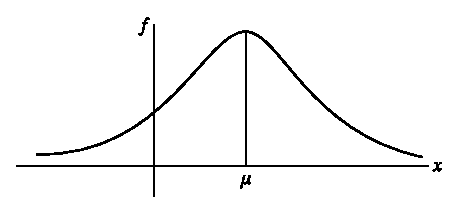
\includegraphics{figure/fig2.eps}}
\end{nonumdefinition}
\end{frame}

\begin{frame}
\begin{nonumdefinition}[Cont.]
$\mu$ is a point of symmetry of $f$ so by Lecture 11, page 15
$$
E(X)=\mu.
$$
(this why this parameter is called $\mu$).

$\sigma^{2}$ measures The ``width'' of the curve

\medskip
\centerline{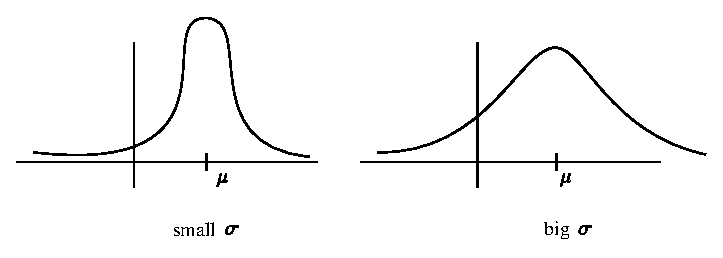
\includegraphics{figure/fig3.eps}}
\end{nonumdefinition}

\begin{nonumproposition}
If $X\sim N(\mu, \sigma^{2})$ then
\begin{itemize}
\item[(i)] $E(X)=\mu$

\item[(ii)] $V(X)=\sigma^{2}$
\end{itemize}
(this justifies the names of the parameters)
\end{nonumproposition}
\end{frame}

\begin{frame}
\begin{nonumremark}
If $X\sim N(\mu,\sigma^{2})$ then
$$
P(a\leq X\leq b)=\int\limits^{b}_{a}\frac{1}{\sqrt{2\pi}\sigma}e^{-\frac{1}{2}(\frac{X-\mu}{\sigma})^{2}}dx
$$
This integral cannot be computed by calculus methods so it must be computed by numerical analysis methods. However these probabilities can be recovered from the table in the front flip text or from a computer. To do this we need to reduce to the ``standard'' case $\mu=0$, $\sigma=1$ (otherwise we would need infinitely many tables, one for each pair $(\mu,\sigma^{2})$). The reduction to the standard case is called \underline{standardization}.
\end{nonumremark}
\end{frame}

\begin{frame}
\myheading{The Standard Normal Distribution}

\begin{nonumdefinition}
A normal distribution with mean $0$ and variance $1$ (so $\mu=0$ and $\sigma^{2}=1$, so $\sigma=1$) is called a \underline{standard normal distribution}.

A random variable with standard normal distribution will be denoted $Z$ so $Z\sim N(0,1)$.

The pdf $f(z)$ for $Z$ is given by
$$
f(z)=\dfrac{1}{\sqrt{2\pi}} e^{-\frac{1}{2}z^{2}}, -\infty < z<-\infty
$$
(see the next page for the graph of $f$)

The function on the right is often called the Gaussian and comes up all over mathematics. It gives rise to the famous theta functions in number theory.
\end{nonumdefinition}
\end{frame}

\begin{frame}
\begin{nonumdefinition}
The cumulative distribution function of the normal distribution will be denoted $\Phi(z)$. So
$$
\Phi(z)=P(Z\leq z)=\int\limits^{z}_{-\infty}\frac{1}{\sqrt{2\pi}}e^{-\frac{1}{2}t^{2}}dt
$$
\end{nonumdefinition}

\myheading{Pictures}

\centerline{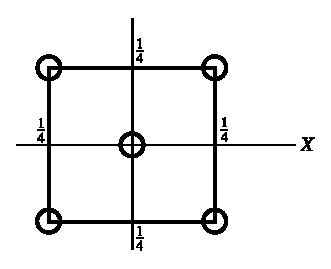
\includegraphics[scale=.85]{figure/fig4.eps}}

\centerline{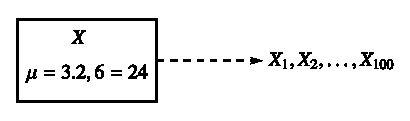
\includegraphics[scale=.9]{figure/fig5.eps}}

\centerline{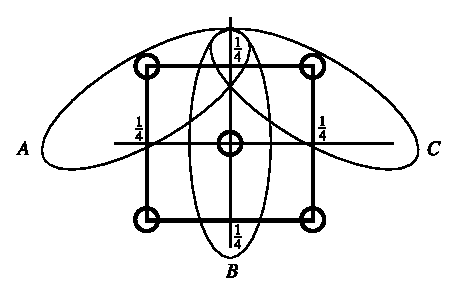
\includegraphics[scale=.9]{figure/fig6.eps}}
\end{frame}

\begin{frame}
$\lim\limits_{z\to -\infty}\Phi(z)=0$

$\lim\limits_{z\to \infty}\Phi(z)=1$

\myheading{Using the tables on page 668-669}

%raghu page 7
\end{frame}

\begin{frame}

\end{frame}

\begin{frame}

\end{frame}

\begin{frame}

\end{frame}

\begin{frame}

\end{frame}

\begin{frame}

\end{frame}

\begin{frame}

\end{frame}

\begin{frame}

\end{frame}

\begin{frame}

\end{frame}

\begin{frame}

\end{frame}

\begin{frame}

\end{frame}

\begin{frame}

\end{frame}

\begin{frame}

\end{frame}

\begin{frame}

\end{frame}

\begin{frame}

\end{frame}

\begin{frame}

\end{frame}

\begin{frame}

\end{frame}

\begin{frame}

\end{frame}

\begin{frame}

\end{frame}

\begin{frame}

\end{frame}

\begin{frame}

\end{frame}

\begin{frame}

\end{frame}

\begin{frame}

\end{frame}

\begin{frame}

\end{frame}

\begin{frame}

\end{frame}

\begin{frame}

\end{frame}

\begin{frame}

\end{frame}

\begin{frame}

\end{frame}

\begin{frame}

\end{frame}

\end{document}


